%=====================µŒ=======ÑÔ==============================
\documentclass[a4paper,12pt]{article}%\documentclass[a4paper,12pt,titlepage]{article}
%======================Include Packages========================
\usepackage[centerlast]{caption2}
\usepackage{fancybox}
\usepackage{amsfonts}
\usepackage[toc,page,title,titletoc,header]{appendix}
\usepackage{color}
\usepackage{titlesec}
\usepackage{ifthen,calc,lastpage,listings}
\usepackage{amsthm}
\usepackage{latexsym}
\usepackage{amsmath}        % AMSLaTeX
\usepackage{amssymb}        % AMSLaTeX sym-bols
\usepackage{indentfirst}    % indent first line of each paragraph
\usepackage{longtable}      % table that occupies multiple pages
\usepackage{subfigure}      %
\usepackage{slashbox}       %@@����ͷ��б��
\usepackage{graphicx}       %@@ͼ��
\usepackage{graphics}       %@@ͼ��
\usepackage[centerlast]{caption2}
\usepackage{flafter}
\usepackage{pifont}
\usepackage{picinpar}
\usepackage{CJK}

%===============��������=============================
\usepackage{mathptmx}  % times roman, including math (where possible)
\usepackage{mathpazo}  % palatino, including math (where possible)
\usepackage{helvet}    % helvetica
%====================================================

\usepackage{colortbl}
\definecolor{grey}{rgb}{0.91,0.91,0.91}

%===========================���嶨��============================
%\DeclareSymbolFont{operators}{OT1}{cmtt}{m}{n}
%\DeclareMathSizes{10}{10}{7}{5}
%\DeclareSymbolFont{symbols}{OMS}{cmex}{m}{n}
%\mathversion{bold}
%\DeclareMathSizes{13.82}{14.4}{10}{7}


% style: page layout
\setlength{\headheight}{15pt}
\setlength{\headsep}{20pt}
\setlength{\footskip}{30pt}
\setlength{\voffset}{-5pt}
\setlength{\hoffset}{16pt}
\setlength{\oddsidemargin}{0pt}
\setlength{\evensidemargin}{\oddsidemargin}
\setlength{\textwidth}{\paperwidth-2\hoffset-2\oddsidemargin-2in}
\setlength{\marginparpush}{0pt}
\setlength{\marginparwidth}{0pt}
\addtolength{\textheight}{3\baselineskip}

% style: float counter
\setcounter{totalnumber}{6}
\setcounter{topnumber}{3}
\setcounter{bottomnumber}{3}

% style: table & figure caption vertical space
\setlength{\abovecaptionskip}{10pt}
\setlength{\belowcaptionskip}{10pt}

% style: table & figure caption font size and face
\renewcommand{\figurename}{\footnotesize{\textbf{Fig}}}
\renewcommand{\tablename}{\footnotesize{\textbf{Tab}}}

% style: table of contents topic depth
\setcounter{tocdepth}{3}

% style: list typesetting
\definecolor{grey}{rgb}{0.3,0.3,0.3}
\definecolor{darkgreen}{rgb}{0,0.3,0}
\definecolor{darkblue}{rgb}{0,0,0.3}
\definecolor{grey}{rgb}{0.95,0.95,0.95}
\definecolor{darkgreen}{rgb}{0.0,0.5078,0.0}

\lstset{language=Matlab}
\lstset{xleftmargin=1em,xrightmargin=1em}
\lstset{frame=}
\lstset{%backgroundcolor=\color{grey},
commentstyle=\color{darkgreen},keywordstyle=\color{blue},%,caption=\lstname,basicstyle=\footnotesize,
breaklines=true,columns=flexible,mathescape=fause }
\lstset{framexleftmargin=0.5em,framexrightmargin=1em,framextopmargin=0em,basicstyle=\footnotesize,framexbottommargin=1em}
%\lstdefinestyle{numbers}{numbers=left,stepnumber=1,numberstyle=\small,numbersep=1em}
\lstloadlanguages{C,C++,Java,Matlab,Mathematica}
%===============================================================%                      %

%===========================Ŀ¼�¶���==========================
\usepackage{titletoc}
\titlecontents{section}[0mm]
{\vspace{.2\baselineskip}\bfseries}
{\normalsize{\thecontentslabel}~\hspace{.5em}} {}
{\dotfill\contentspage[{\makebox[0pt][r]{\thecontentspage}}]}
[\vspace{.1\baselineskip}]
\dottedcontents{section}[1.16cm]{\large}{2.0em}{4pt}
\dottedcontents{subsection}[2.00cm]{\normalsize}{2.0em}{4pt}
%===============================================================

%=========================¶šÒåҳÌ================================
\usepackage{fancyhdr}
\pagestyle{fancy} \lhead{Page \thepage\ of \pageref{LastPage}}
\chead{} \rhead{Team \footnotesize{\#} 17617}
\cfoot{\thepage}%%% team control number as package option    @@ ÐÞž% XeLaTeX can use any Mac OS X font. See the setromanfont command below.
% Input to XeLaTeX is full Unicode, so Unicode characters can be typed directly into the source.

% The next lines tell TeXShop to typeset with xelatex, and to open and save the source with Unicode encoding.

%!TEX TS-program = xelatex
%!TEX encoding = UTF-8 Unicode

\documentclass[12pt]{article}
\usepackage{geometry}                % See geometry.pdf to learn the layout options. There are lots.
\geometry{letterpaper}                   % ... or a4paper or a5paper or ... 
%\geometry{landscape}                % Activate for for rotated page geometry
%\usepackage[parfill]{parskip}    % Activate to begin paragraphs with an empty line rather than an indent
\usepackage{graphicx}
\usepackage{amssymb}

% Will Robertson's fontspec.sty can be used to simplify font choices.
% To experiment, open /Applications/Font Book to examine the fonts provided on Mac OS X,
% and change "Hoefler Text" to any of these choices.

\usepackage{fontspec,xltxtra,xunicode}
\defaultfontfeatures{Mapping=tex-text}
\setromanfont[Mapping=tex-text]{Hoefler Text}
\setsansfont[Scale=MatchLowercase,Mapping=tex-text]{Gill Sans}
\setmonofont[Scale=MatchLowercase]{Andale Mono}

\title{Brief Article}
\author{The Author}
%\date{}                                           % Activate to display a given date or no date

\begin{document}
\maketitle

% For many users, the previous commands will be enough.
% If you want to directly input Unicode, add an Input Menu or Keyboard to the menu bar 
% using the International Panel in System Preferences.
% Unicode must be typeset using a font containing the appropriate characters.
% Remove the comment signs below for examples.

% \newfontfamily{\A}{Geeza Pro}
% \newfontfamily{\H}[Scale=0.9]{Lucida Grande}
% \newfontfamily{\J}[Scale=0.85]{Osaka}

% Here are some multilingual Unicode fonts: this is Arabic text: {\A السلام عليكم}, this is Hebrew: {\H שלום}, 
% and here's some Japanese: {\J 今日は}.



\end{document}  % XeLaTeX can use any Mac OS X font. See the setromanfont command below.
% Input to XeLaTeX is full Unicode, so Unicode characters can be typed directly into the source.

% The next lines tell TeXShop to typeset with xelatex, and to open and save the source with Unicode encoding.

%!TEX TS-program = xelatex
%!TEX encoding = UTF-8 Unicode

\documentclass[12pt]{article}
\usepackage{geometry}                % See geometry.pdf to learn the layout options. There are lots.
\geometry{letterpaper}                   % ... or a4paper or a5paper or ... 
%\geometry{landscape}                % Activate for for rotated page geometry
%\usepackage[parfill]{parskip}    % Activate to begin paragraphs with an empty line rather than an indent
\usepackage{graphicx}
\usepackage{amssymb}

% Will Robertson's fontspec.sty can be used to simplify font choices.
% To experiment, open /Applications/Font Book to examine the fonts provided on Mac OS X,
% and change "Hoefler Text" to any of these choices.

\usepackage{fontspec,xltxtra,xunicode}
\defaultfontfeatures{Mapping=tex-text}
\setromanfont[Mapping=tex-text]{Hoefler Text}
\setsansfont[Scale=MatchLowercase,Mapping=tex-text]{Gill Sans}
\setmonofont[Scale=MatchLowercase]{Andale Mono}

\title{Brief Article}
\author{The Author}
%\date{}                                           % Activate to display a given date or no date

\begin{document}
\maketitle

% For many users, the previous commands will be enough.
% If you want to directly input Unicode, add an Input Menu or Keyboard to the menu bar 
% using the International Panel in System Preferences.
% Unicode must be typeset using a font containing the appropriate characters.
% Remove the comment signs below for examples.

% \newfontfamily{\A}{Geeza Pro}
% \newfontfamily{\H}[Scale=0.9]{Lucida Grande}
% \newfontfamily{\J}[Scale=0.85]{Osaka}

% Here are some multilingual Unicode fonts: this is Arabic text: {\A السلام عليكم}, this is Hebrew: {\H שלום}, 
% and here's some Japanese: {\J 今日は}.



\end{document}  

\end% XeLaTeX can use any Mac OS X font. See the setromanfont command below.
% Input to XeLaTeX is full Unicode, so Unicode characters can be typed directly into the source.

% The next lines tell TeXShop to typeset with xelatex, and to open and save the source with Unicode encoding.

%!TEX TS-program = xelatex
%!TEX encoding = UTF-8 Unicode

\documentclass[12pt]{article}
\usepackage{geometry}                % See geometry.pdf to learn the layout options. There are lots.
\geometry{letterpaper}                   % ... or a4paper or a5paper or ... 
%\geometry{landscape}                % Activate for for rotated page geometry
%\usepackage[parfill]{parskip}    % Activate to begin paragraphs with an empty line rather than an indent
\usepackage{graphicx}
\usepackage{amssymb}

% Will Robertson's fontspec.sty can be used to simplify font choices.
% To experiment, open /Applications/Font Book to examine the fonts provided on Mac OS X,
% and change "Hoefler Text" to any of these choices.

\usepackage{fontspec,xltxtra,xunicode}
\defaultfontfeatures{Mapping=tex-text}
\setromanfont[Mapping=tex-text]{Hoefler Text}
\setsansfont[Scale=MatchLowercase,Mapping=tex-text]{Gill Sans}
\setmonofont[Scale=MatchLowercase]{Andale Mono}

\title{Brief Article}
\author{The Author}
%\date{}                                           % Activate to display a given date or no date

\begin{document}
\maketitle

% For many users, the previous commands will be enough.
% If you want to directly input Unicode, add an Input Menu or Keyboard to the menu bar 
% using the International Panel in System Preferences.
% Unicode must be typeset using a font containing the appropriate characters.
% Remove the comment signs below for examples.

% \newfontfamily{\A}{Geeza Pro}
% \newfontfamily{\H}[Scale=0.9]{Lucida Grande}
% \newfontfamily{\J}[Scale=0.85]{Osaka}

% Here are some multilingual Unicode fonts: this is Arabic text: {\A السلام عليكم}, this is Hebrew: {\H שלום}, 
% and here's some Japanese: {\J 今日は}.



\end{document}  ĶӺÅ
\rfoot{}
\renewcommand{\headrulewidth}{0pt}% XeLaTeX can use any Mac OS X font. See the setromanfont command below.
% Input to XeLaTeX is full Unicode, so Unicode characters can be typed directly into the source.

% The next lines tell TeXShop to typeset with xelatex, and to open and save the source with Unicode encoding.

%!TEX TS-program = xelatex
%!TEX encoding = UTF-8 Unicode

\documentclass[12pt]{article}
\usepackage{geometry}                % See geometry.pdf to learn the layout options. There are lots.
\geometry{letterpaper}                   % ... or a4paper or a5paper or ... 
%\geometry{landscape}                % Activate for for rotated page geometry
%\usepackage[parfill]{parskip}    % Activate to begin paragraphs with an empty line rather than an indent
\usepackage{graphicx}
\usepackage{amssymb}

% Will Robertson's fontspec.sty can be used to simplify font choices.
% To experiment, open /Applications/Font Book to examine the fonts provided on Mac OS X,
% and change "Hoefler Text" to any of these choices.

\usepackage{fontspec,xltxtra,xunicode}
\defaultfontfeatures{Mapping=tex-text}
\setromanfont[Mapping=tex-text]{Hoefler Text}
\setsansfont[Scale=MatchLowercase,Mapping=tex-text]{Gill Sans}
\setmonofont[Scale=MatchLowercase]{Andale Mono}

\title{Brief Article}
\author{The Author}
%\date{}                                           % Activate to display a given date or no date

\begin{document}
\maketitle

% For many users, the previous commands will be enough.
% If you want to directly input Unicode, add an Input Menu or Keyboard to the menu bar 
% using the International Panel in System Preferences.
% Unicode must be typeset using a font containing the appropriate characters.
% Remove the comment signs below for examples.

% \newfontfamily{\A}{Geeza Pro}
% \newfontfamily{\H}[Scale=0.9]{Lucida Grande}
% \newfontfamily{\J}[Scale=0.85]{Osaka}

% Here are some multilingual Unicode fonts: this is Arabic text: {\A السلام عليكم}, this is Hebrew: {\H שלום}, 
% and here's some Japanese: {\J 今日は}.



\end{document}  
%==================================================================
\usepackage[dvipdfm,colorlinks=true]{hyperref}
\graphicspath{{figures/}}
%==========================µŒÑÔ¶šÒåœáÊø============================

%%%%%%%%%%%%%%%%%%%%%%%%%%%%%%%%%%%%%%%%%%%%%%%%%%%%%%%%%%%%%%%%%%%
%%%%%%%%%%%%%%%%%%$$$$$$$==ÕýÎÄ¿ªÊŒ==$$$$$$$%%%%%%%%%%%%%%%%%%%%%%%
%%%%%%%%%%%%%%%%%%%%%%%%%%%%%%%%%%%%%%%%%%%%%%%%%%%%%%%%%%%%%%%%%%%

%==========================ÂÛÎıêÌâ===============================
\title{\rmfamily{\textbf{The Newest \LaTeX{} Template for MCM}}}
%\author{Team 17617}
%=================================================================
%==================================================================
\begin{document}
\maketitle
%\thispagestyle{empty}
%==================================================================

%\vspace*{\fill}
%====================Õª=======Òª===================================
\input{abstract.tex}                                              %
\newpage                                                          %
%==================================================================


%====================Éú=³É=Ä¿=ÂŒ===================================
\tableofcontents                                                  %
\thispagestyle{plain}                                             %
\newpage                                                          %
%==================================================================

%======================�������====================================
\section{Introduction}

Although a hitter might expect a model of the bat�Cbaseball collision to
yield insight into how the bat breaks, how the bat imparts spin on the ball,
how best to swing the bat, and so on, we model only the sweet spot.

There are at least two notions of where the sweet spot should be��an
impact location on the bat that either
\begin{itemize}
\item minimizes the discomfort to the hands, or
\item maximizes the outgoing velocity of the ball.
\end{itemize}
We focus exclusively on the second definition.

\begin{itemize}
  \item the initial velocity and rotation of the ball,
\item the initial velocity and rotation of the bat,
\item the relative position and orientation of the bat and ball, and
\item the force over time that the hitter�s hands applies on the handle.
\end{itemize}
We assume that the ball is not rotating and that its velocity at impact is
perpendicular to the length of the bat. We assume that everything occurs
in a single plane, and we will argue that the hands� interaction is negligible.
In the frame of reference of the center of mass of the bat, the initial conditions
are completely specified by
\begin{itemize}
  \item the angular velocity of the bat,
\item the velocity of the ball, and
\item the position of impact along the bat.
\end{itemize}
The location of the sweet spot depends not on just the bat alone but also
on the pitch and on the swing.
The simplest model for the physics involved has the sweet spot at the
\emph{center of percussion} [Brody 1986], the impact location that minimizes discomfort
to the hand. The model assumes the ball to be a rigid body for which
there are conjugate points: An impact at one will exactly balance the angular
recoil and linear recoil at the other. By gripping at one and impacting at the
other (the center of percussion), the hands experience minimal shock and
the ball exits with high velocity. The center of percussion depends heavily
on the moment of inertia and the location of the hands. We cannot accept
this model because it both erroneously equates the two definitions of sweet
spot and furthermore assumes incorrectly that the bat is a rigid body.
Another model predicts the sweet spot to be between nodes of the two
lowest natural frequencies of the bat [Nathan 2000]. Given a free bat allowed
to oscillate, its oscillations can be decomposed into fundamental
modes of various frequencies. Different geometries and materials have different
natural frequencies of oscillation. The resulting wave shapes suggest
how to excite those modes (e.g., plucking a string at the node of a vibrational
mode will not excite that mode).




    \begin{Theorem} \label{thm:latex}
    \LaTeX 
    \end{Theorem}
    \begin{Lemma} \label{thm:tex}
    \TeX .
    \end{Lemma}
    \begin{proof}
    The proof of theorem.
    \end{proof}






\subsection{Other Assumptions}
%\renewcommand{\labelitemi}{\ding{43}}
Although Mr. Gore has expressed concerns to some associates about
the damage a brokered convention could cause, several associates
said he was hopeful that one candidate would soon break through,
sparing the party such an outcome. He told a close friend recently
that his decision not to endorse ��feels like the right thing��
and that he remained optimistic the race ��is going to tip at some
point,�� the friend said.
\begin{itemize}
\item
\item
\item
\item
\end{itemize}

 Under the above and basic assumptions, we can set out
to construct our model (show our approach in detail).
%=============================�������==========================================
\section{Analysis of the Problem }
%==================================ģ�ͽ���==============================================
\begin{figure}[h]
\small
\centering
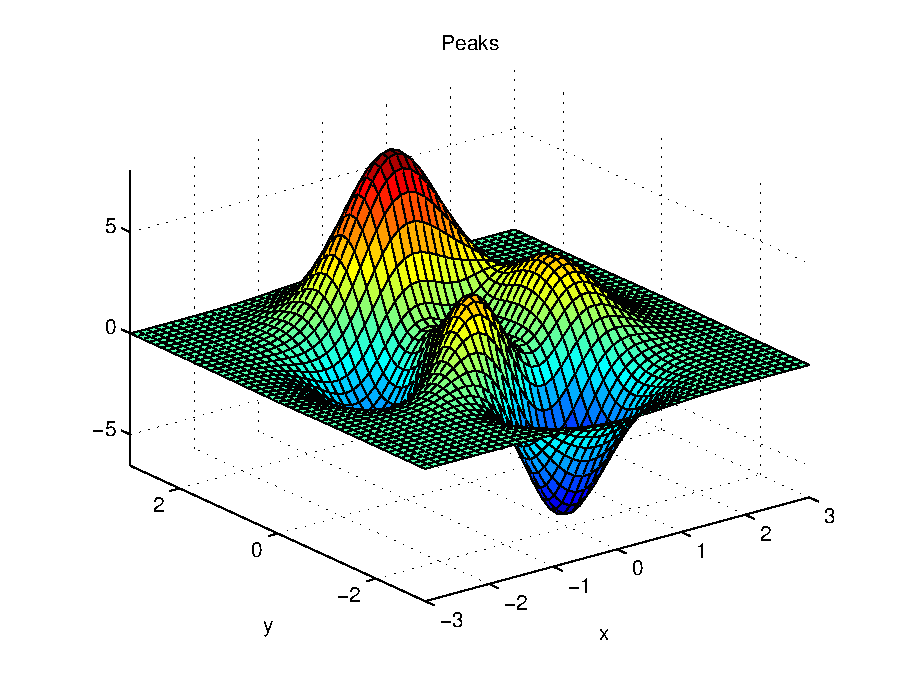
\includegraphics[width=12cm]{./picture/aaa.eps}
\caption{aa} \label{fig:aa}
\end{figure}

Although Mr. Gore has expressed concerns to some associates about
the damage a brokered convention could cause, several associates
said he was hopeful that one candidate would soon break through,
sparing the party such an outcome. He told a close friend recently
that his decision not to endorse ��feels like the right thing��
and that he remained optimistic the race ��is going to tip at some
point,�� the friend said.\eqref{aa}
\begin{equation}
  a^2 \label{aa}
\end{equation}


\[
\left( {\begin{array}{*{20}c}
   {a_{11} } & {a_{12} } & {a_{13} }  \\
   {a_{21} } & {a_{22} } & {a_{23} }  \\
   {a_{31} } & {a_{32} } & {a_{33} }  \\
\end{array}} \right) = \frac{{Opposite}}{{Hypotenuse}}\cos ^{ - 1} \theta \arcsin \theta
\]
Although Mr. Gore has expressed concerns to some associates about
the damage a brokered convention could cause, several associates
said he was hopeful that one candidate would soon break through,
sparing the party such an outcome. He told a close friend recently
that his decision not to endorse ��feels like the right thing��
and that he remained optimistic the race ��is going to tip at some
point,�� the friend said.

\[
p_{j}=\begin{cases} 0,&\text{if $j$ is odd}\\
r!\,(-1)^{j/2},&\text{if $j$ is even}
\end{cases}
\]
Although Mr. Gore has expressed concerns to some associates about
the damage a brokered convention could cause, several associates
said he was hopeful that one candidate would soon break through,
sparing the party such an outcome. He told a close friend recently
that his decision not to endorse ��feels like the right thing��
and that he remained optimistic the race ��is going to tip at some
point,�� the friend said.
\[
\arcsin \theta  =
\mathop{{\int\!\!\!\!\!\int\!\!\!\!\!\int}\mkern-31.2mu
\bigodot}\limits_\varphi
 {\mathop {\lim }\limits_{x \to \infty } \frac{{n!}}{{r!\left( {n - r}
 \right)!}}} \eqno (1)
\]




\section{Calculating and Simplifying the Model  } ``A is equivalent
to B'' Although Mr. Gore has expressed concerns to some associates
about the damage a brokered convention could cause, several
associates said he was hopeful that one candidate would soon break
through, sparing the party such an outcome. He told a close friend
recently that his decision not to endorse ��feels like the right
thing�� and that he remained optimistic the race ��is going to tip
at some point,�� the friend said.



%===============================ģ�ͽ��============================================
\section{The Model Results}
Although Mr. Gore has expressed concerns to some associates about
the damage a brokered convention could cause, several associates
said he was hopeful that one candidate would soon break through,
sparing the party such an outcome. He told a close friend recently
that his decision not to endorse ��feels like the right thing��
and that he remained optimistic the race ��is going to tip at some
point,�� the friend said.


%========================ģ�͵�ʵЧ��������Ӧ��˵����=============================

\section{Validating the Model}%ȷ��ģ�ͣ�ʹ֮������
Although Mr. Gore has expressed concerns to some associates about
the damage a brokered convention could cause, several associates
said he was hopeful that one candidate would soon break through,
sparing the party such an outcome. He told a close friend recently
that his decision not to endorse ��feels like the right thing��
and that he remained optimistic the race ��is going to tip at some
point,�� the friend said. Although Mr. Gore has expressed concerns
to some associates about the damage a brokered convention could
cause, several associates said he was hopeful that one candidate
would soon break through, sparing the party such an outcome. He
told a close friend recently that his decision not to endorse
��feels like the right thing�� and that he remained optimistic the
race ��is going to tip at some point,�� the friend said.


Although Mr. Gore has expressed concerns to some associates about
the damage a brokered convention could cause, several associates
said he was hopeful that one candidate would soon break through,
sparing the party such an outcome. He told a close friend recently
that his decision not to endorse ��feels like the right thing��
and that he remained optimistic the race ��is going to tip at some
point,�� the friend said.

\section{Conclusions}
Although Mr. Gore has expressed concerns to some associates about
the damage a brokered convention could cause, several associates
said he was hopeful that one candidate would soon break through,
sparing the party such an outcome. He told a close friend recently
that his decision not to endorse ��feels like the right thing��
and that he remained optimistic the race ��is going to tip at some
point,�� the friend said.
\section{A Summary    }
Although Mr. Gore has expressed concerns to some associates about
the damage a brokered convention could cause, several associates
said he was hopeful that one candidate would soon break through,
sparing the party such an outcome. He told a close friend recently
that his decision not to endorse ��feels like the right thing��
and that he remained optimistic the race ��is going to tip at some
point,�� the friend said.
%================================��������==============================
\section{Evaluate of the Mode}

%======================================================================
\section{Strengths and weaknesses}
Like any model,the one present above has its strengths and
weaknesses. Some of the major points are presented below.

%============================ģ��=�ŵ�====================================
\subsection{Strengths}
\begin{itemize}
\item \textbf{Applies widely}\\
This  system can be used for many types of airplanes, and it also
solves the interference during  the procedure of the boarding
airplane,as described above we can get to the  optimization
boarding time.We also know that all the service is automate.
\item \textbf{Improve the quality of the airport service}\\
Balancing the cost of the cost and the benefit, it will bring in
more convenient  for airport and passengers.It also saves many
human resources for the airline. \item \textbf{}
\end{itemize}




\begin{thebibliography}{99}
\addcontentsline{toc}{section}{References}
\bibitem[D. E. KNUTH]{1} D. E. KNUTH   The \TeX{}book  the American
Mathematical Society and Addison�CWesley
Publishing Company , 1984-1986.
\bibitem{2}Lamport, Leslie,  \LaTeX{}: `` A Document Preparation System '',
Addison-Wesley Publishing Company, 1986.
\end{thebibliography}

%====================��¼����������==========================================
    \begin{appendices}
    %\renewcommand{\thesection}{\Alph{chapter}.}

      \section{First appendix}

    some text...


Here are simulation programmes we used in our model as follow.\\


\textbf{\textcolor[rgb]{0.98,0.00,0.00}{Input matlab source:}}
\lstinputlisting[language=Matlab]{./code/matlab1.m}


      \section{Second appendix}

    some more text\textcolor[rgb]{0.98,0.00,0.00}{\textbf{Input C++ source:}}
\lstinputlisting[language=C++]{./code/sudoku.cpp}

    \end{appendices} 


\end{document}
%%%%%%%%%%%%%%%%%%%%%%%%%%%%%%%%%%%%%%%%%%%%%%%%%%%%%%%%%%%%%%%%%%%
%%%%%%%%%%===========THE END OF PAPER============%%%%%%%%%%%%%%%%%%
%%%%%%%%%%%%%%%%%%%%%%%%%%%%%%%%%%%%%%%%%%%%%%%%%%%%%%%%%%%%%%%%%%%
